\begingroup
\thispagestyle{empty}
\begin{tikzpicture}[remember picture,overlay]
\coordinate [below=5 cm] (midpoint) at (current page.north);
\node at (current page.north west)
{\begin{tikzpicture}[remember picture,overlay]
\node[anchor=north west,inner sep=0pt] at (0,0) {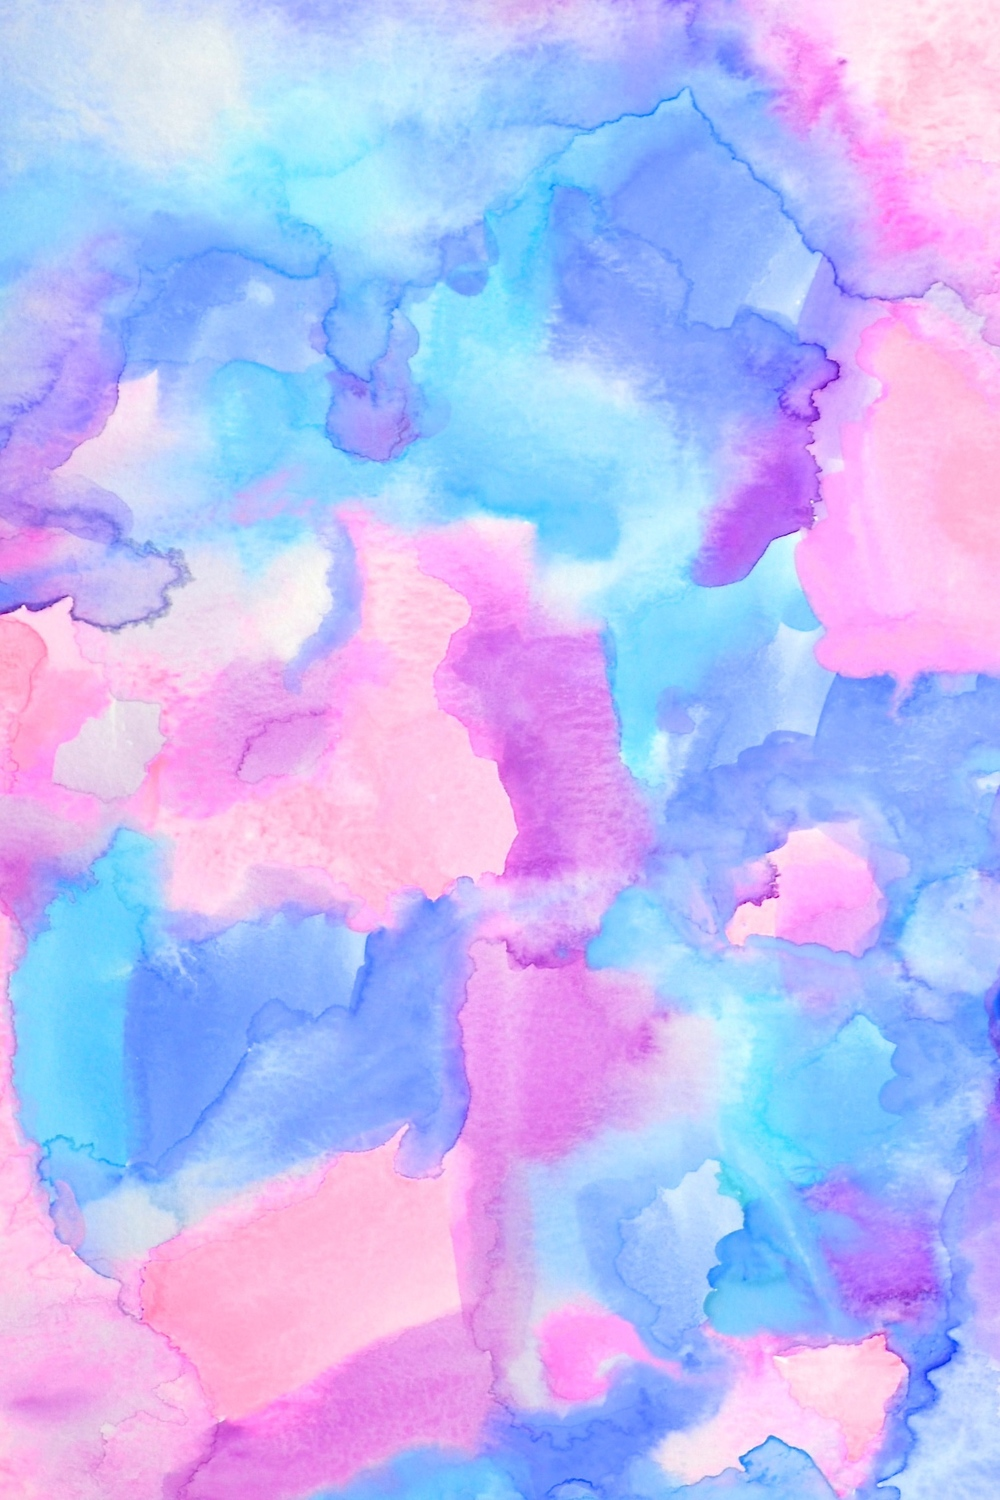
\includegraphics[width=\paperwidth]{pictures/background}}; % Background image
\draw[anchor=north] (midpoint) node [fill=prpl!30!white,fill opacity=0.6,text opacity=1,inner sep=0.8cm]{\Huge\centering\bfseries\sffamily\parbox[c][][t]{\paperwidth}{\centering { \textcolor{black!70}{\fontsize{23}{14}\selectfont GOSBook}}\\[4pt] % Book title
%{\Large }\\[20pt] % Subtitle
{\textcolor{black!70}{\huge Didenko Andr\'e}}\\[2pt] % Author name
{\textcolor{black!70}{\LARGE\scshape Edition from \twodigit\day.\twodigit\month.\the\year}}}}; 
\end{tikzpicture}};
\end{tikzpicture}
\vfill

%\shadetext[left color=CornflowerBlue, right color=prpl, middle color=prpl, shading angle=55]{\huge Didenko Andre}

\newpage
\thispagestyle{empty}
\epigraph{Умереть не страшно, страшно не жить.}{Виктор Гюго}\centering
\vspace*{-0.7\baselineskip}  
\settowidth{\unitlength}{\LARGE\scshape Московский Физико"--~Технический Институт}
\begin{figure}[!h]
\center
\includegraphics[width=0.18\textwidth]{pictures/MIPT2}
\vspace{-0.5\baselineskip}
\end{figure}
{\LARGE\scshape Московский Физико"--~Технический Институт}
\rule{\unitlength}{1.7pt}\vspace*{-\baselineskip}\vspace*{2pt}
\rule{\unitlength}{0.4pt}\\[0.6\baselineskip]
{\Huge Подготовка к ГОСу по Матану}\\[0.4\baselineskip]
{\large \itshape Sapere aude}\\[0.14\baselineskip]
\rule{\unitlength}{0.4pt}\vspace*{-1.5\baselineskip}\vspace{3.2pt}
\rule{\unitlength}{1.7pt}\\[0.55\baselineskip]
{\Large\scshape Диденко А.А. \\\vspace*{0.1\baselineskip}  \normalsize студент 311 группы}\par
\vspace*{0.35\baselineskip}  

{\LARGE\scshape Редакция от \twodigit\day.\twodigit\month.\the\year \;(\currenttime)}\par 

\vspace*{-1\baselineskip}  
\begin{flushleft}
\section*{\Large Полезные ссылки}
\begin{itemize}[wide, labelwidth=!, labelindent=0pt, label=$\blacktriangleright$, noitemsep]
\item Последняя версия книги в pdf-формате всегда доступна по ссылке:

\qquad\href{https://didenkoandre.github.io/GOSBook/GOSBook.pdf}{$
\begin{array}{l}

\includegraphics[width=\iconwidth]{pictures/reference/favicon}
\end{array}
$\large didenkoandre.github.io/GOSBook/GOSBook.pdf}

\item Web-site, посвященный данной книге:

\qquad\href{https://didenkoandre.github.io/GOSBook}{$
\begin{array}{l}

\includegraphics[width=\iconwidth]{pictures/reference/favicon}
\end{array}
$\large didenkoandre.github.io/GOSBook}
\iffalse
\qquad\href{http://latexonline.cc/compile?git=https://github.com/DidenkoAndre/GOSBook&target=GOSBook.tex&download=GOSBook.pdf&command=pdflatex}{$
\begin{array}{l}

\includegraphics[width=\iconwidth]{pictures/reference/latexonline}
\end{array}
$\large latexonline.cc/...}

\qquad\href{https://www.dropbox.com/s/nly4ewbfcyrc8es/GOSBook.pdf?dl=0}{$
\begin{array}{l}

\includegraphics[width=\iconwidth]{pictures/reference/dropbox}
\end{array}
$\large dropbox.com/...}
\fi

\item Дополнительные материалы, полезные при подготовке как к \textit{устному} экзамену, так и к \textit{письменному} доступны по ссылке:

\qquad\href{https://drive.google.com/drive/u/0/folders/0BzuzEyNkpwYDYjVNcE0wa3hqWjA}{$
\begin{array}{l}

\includegraphics[width=\iconwidth]{pictures/reference/drive}
\end{array}
$\large drive.google.com/...}

\item Литература по курсам доступна по ссылке:

\qquad\href{https://drive.google.com/drive/u/0/folders/0BzuzEyNkpwYDcENXcV9jNWdwVlU}{$
\begin{array}{l}

\includegraphics[width=\iconwidth]{pictures/reference/drive}
\end{array}
$\large drive.google.com/...}

\item Анкета о ГОСе, которую рекомендую всем заполнить после его сдачи:

\qquad\href{https://docs.google.com/spreadsheets/d/10jIg9Nr5oM1-Zjo_iIlKs8uxrBKrzfuJNas_YJIIxPs/edit\#gid=0}{$
\begin{array}{l}

\includegraphics[width=\iconwidth]{pictures/reference/drive}
\end{array}
$\large drive.google.com/...}

\iffalse
\item Подпишитесь на наш Telegram-бот с помощью команды \textsf{/subscribe}, и вы будете получать свежую версию автоматически!

\qquad\href{https://t.me/gosbook_bot}{$
\begin{array}{l}

\includegraphics[width=\iconwidth]{pictures/reference/telegram}
\end{array}
$\large /GOSBook\_Bot} 
\fi

\item Репозиторий, в котором хранится этот документ:

\qquad\href{https://github.com/DidenkoAndre/GOSBook}{$
\begin{array}{l}

\includegraphics[width=\iconwidth]{pictures/reference/git}
\end{array}
$\large /didenkoandre/GOSBook}

\iffalse
\item Вы всегда можете поддержать проект материально! 
Перевести средства на развитие проекта можно на карту {\large 5244 6873 8510 3816} \textsf{(MasterCard)}.
\fi

\item По любым вопросам касательно книги, а также если вы хотите помочь в написании материала, просьба обращаться в личные сообщения: 

\qquad\href{https://vk.com/didenko_andre}{$
\begin{array}{l}

\includegraphics[width=\iconwidth]{pictures/reference/vk}
\end{array}
$\large /didenko\_\!andre}

\qquad\href{https://t.me/didenko_andre}{$
\begin{array}{l}

\includegraphics[width=\iconwidth]{pictures/reference/telegram}
\end{array}
$\large /didenko\_\!andre}

\qquad\href{https://instagram.com/didenko_andre}{$
    \begin{array}{l}
    
\includegraphics[width=\iconwidth]{pictures/reference/instagram}
    \end{array}
$\large /didenko\_\!andre}
\vspace*{-1\baselineskip}  
\end{itemize}

\section*{\Large Текущий статус книги}

$\blacktriangleright$ В данный момент потихоньку переписываю книгу к новой программе 2018 года и совершенствую остальной материал.

\smallskip

\vfill

\textcolor{red}{
$\blacktriangleright$ Я крайне не рекомендую использовать данное пособие как \textit{\textbf{основную}} литературу во время подготовки к Государственному экзамену.
}

\end{flushleft}

\medskip
\vfill
{\huge\scshape I\;$\heartsuit$\;\LaTeX}\\[0.5\baselineskip]
{\LARGE\scshape 2016}\par
\restoregeometry
\endgroup
\newpage